%%%%%%%%%%%%%%%%%%%%%%%%%%%%%%%%%%%%%%%%%
% Beamer Presentation
% LaTeX Template
% Version 1.0 (10/11/12)
%
% This template has been downloaded from:
% http://www.LaTeXTemplates.com
%
% License:
% CC BY-NC-SA 3.0 (http://creativecommons.org/licenses/by-nc-sa/3.0/)
%
%%%%%%%%%%%%%%%%%%%%%%%%%%%%%%%%%%%%%%%%%

%----------------------------------------------------------------------------------------
%	PACKAGES AND THEMES
%----------------------------------------------------------------------------------------

\documentclass{beamer}


\mode<presentation> {

% The Beamer class comes with a number of default slide themes
% which change the colors and layouts of slides. Below this is a list
% of all the themes, uncomment each in turn to see what they look like.

\usetheme{default}

\usefonttheme{serif} % default family is serif

%\usetheme{AnnArbor}
%\usetheme{Antibes}
%\usetheme{Bergen}
%\usetheme{Berkeley}
%\usetheme{Berlin}
%\usetheme{Boadilla}
%\usetheme{CambridgeUS}
%\usetheme{Copenhagen}
%\usetheme{Darmstadt}
%\usetheme{Dresden}
%\usetheme{Frankfurt}
%\usetheme{Goettingen}
%\usetheme{Hannover}
%\usetheme{Ilmenau}
%\usetheme{JuanLesPins}
%\usetheme{Luebeck}
%\usetheme{Madrid}
%\usetheme{Malmoe}
%\usetheme{Marburg}
%\usetheme{Montpellier}
%\usetheme{PaloAlto}
%\usetheme{Pittsburgh}
%\usetheme{Rochester}
%\usetheme{Singapore}
%\usetheme{Szeged}
%\usetheme{Warsaw}

% As well as themes, the Beamer class has a number of color themes
% for any slide theme. Uncomment each of these in turn to see how it
% changes the colors of your current slide theme.

%\usecolortheme{albatross}
%\usecolortheme{beaver}
%\usecolortheme{beetle}
%\usecolortheme{crane}
%\usecolortheme{dolphin}
%\usecolortheme{dove}
%\usecolortheme{fly}
%\usecolortheme{lily}
%\usecolortheme{orchid}
%\usecolortheme{rose}
%\usecolortheme{seagull}
%\usecolortheme{seahorse}
%\usecolortheme{whale}
%\usecolortheme{wolverine}

%\setbeamertemplate{footline} % To remove the footer line in all slides uncomment this line
%\setbeamertemplate{footline}[page number] % To replace the footer line in all slides with a simple slide count uncomment this line

%\setbeamertemplate{navigation symbols}{} % To remove the navigation symbols from the bottom of all slides uncomment this line
}

\usepackage{graphicx} % Allows including images
\usepackage{booktabs} % Allows the use of \toprule, \midrule and \bottomrule in tables
\usepackage{multicol}
\usepackage{scrextend}
\usepackage{subfig}

\newcommand{\dd}{\mathrm{d}}
\newcommand{\thetaxy}{\theta_{X|Y }}
\newcommand{\thetayx}{\theta_{Y|X}}

\newcommand{\Nxy}{{N_{X|Y}}}
\newcommand{\Nyx}{{N_{Y|X}}}
\newcommand{\Nyy}{{N_{Y|Y}}}
\newcommand{\Nxx}{{N_{X|X}}}

\newcommand{\dxy}{{\delta_{X|Y}}}
\newcommand{\dyx}{{\delta_{Y|X}}}
\newcommand{\dyy}{{\delta_{Y|Y}}}
\newcommand{\dxx}{{\delta_{X|X}}}
\newcommand{\X}{\textcolor{red}{X}}
\newcommand{\Y}{\textcolor{blue}{Y}}

\definecolor{darkpurple}{rgb}{0.4,0.,0.4}

\usepackage{tcolorbox}

\definecolor{mycolor}{rgb}{0.122, 0.435, 0.698}

\usepackage{tcolorbox}
\newtcolorbox{mybox}{colback=mycolor!5!white,colframe=mycolor!75!black}




\newtcolorbox{mybox1}[1]{colback=blue!5!white,colframe=blue!75!black,fonttitle=\bfseries,title=#1}

\newtcolorbox{mybox2}[1]{colback=green!5!white,colframe=green!75!black,fonttitle=\bfseries,title=#1}

\newtcolorbox{mybox3}[1]{colback=red!5!white,colframe=red!75!black,fonttitle=\bfseries,title=#1}


\usepackage{multimedia}    
\usepackage{lipsum}


%\usepackage[hang,small]{caption}
%----------------------------------------------------------------------------------------
%	TITLE PAGE
%----------------------------------------------------------------------------------------

%\title[Short title]{Eigenfunction expansion of the refractory density for renewal processes} % The short title appears at the bottom of every slide, the full title is only on the title page

\title[Short title]{Low-dimensional population dynamics of spiking neurons via eigenfunction expansion}


\author{No\'e Gallice \\ \medskip Professors:  Wulfram Gerstner and Matthieu Wyart\\ \medskip Supervisor:  Tilo Schwalger} % Your name
\institute[EPFL] % Your institution as it will appear on the bottom of every slide, may be shorthand to save space
{ Laboratory of Computational Neuroscience, EPFL \\ % Your institution for the title page
\medskip % Your email address
}
% Date, can be changed to a custom date
\date{April 23, 2018}

\titlegraphic{
\includegraphics[width=2.5cm]{epfl}\hspace*{4.75cm}~%
	
\includegraphics[width=2cm]{lcn}
}

\begin{document}

\begin{frame}
	\titlepage % Print the title page as the first slide
\end{frame}


\begin{frame}

\small{
	\begin{columns}
	\begin{column}{.12\textwidth}

		
	\end{column}
	\begin{column}{.28\textwidth}
			\centering
		\textbf{Complex system } 
		
	\end{column}
	\begin{column}{.3\textwidth}
			\centering
\textbf{Simplified model} 
	
\end{column}
	\begin{column}{.3\textwidth}
			\centering
		\textbf{Math. tractable / comput. efficiency}
	\end{column}
\end{columns}

\vspace{0.5cm}

\begin{columns}
	\begin{column}{.15\textwidth}
		\textit{Neuron:}
		
	\end{column}
	\begin{column}{.25\textwidth}
	\centering
	Biophysical model 	
	\end{column}
	\begin{column}{.3\textwidth}
	\centering
	Hodgkin-Huxley model 
	\end{column}
	\begin{column}{.3\textwidth}
	\centering
	IF model
	\end{column}
\end{columns}

\pause
\vspace{0.5cm}
\begin{columns}
	\begin{column}{.15\textwidth}
		\textit{Neuronal network:} 
		
	\end{column}
	\begin{column}{.25\textwidth}
		\centering
	Spiking network
	\end{column}
	\begin{column}{.3\textwidth}
		\centering
	  Population density equation
	\end{column}
	\begin{column}{.3\textwidth}
		\centering
		\textcolor{red}{Firing rate model}
	\end{column}
\end{columns}
}

\pause
\vspace{1.2cm}
M. Mattia, P. Del Giudice,  \textit{Phys. Review} (2002)

They derived a low dynamics of the collective firing rate from the spectral expansion of the Fokker-Plank equation.

\vspace{0.8cm}
\pause
\begin{mybox}
	\textbf{Aim: } Derive a low dimensional dynamics taking into account the slowest modes of the expansion of the refractory density.

\end{mybox}

\end{frame}



\begin{frame}
\frametitle{Overview}% Table of contents slide, comment this block out to remove it
\tableofcontents % Throughout your presentation, if you choose to use \section{} and \subsection{} commands, these will automatically be printed on this slide as an overview of your presentation
\end{frame}

%----------------------------------------------------------------------------------------
%	PRESENTATION SLIDES
%----------------------------------------------------------------------------------------

%------------------------------------------------

\setbeamerfont{framesubtitle}{size=\normalsize }

\section{1. Theory}
\subsection{1.1 Refractory density equation}

\begin{frame}
\frametitle{1. Theory}
\framesubtitle{1.1 Refractory density equation}
%We consider a large homogeneous population of neurons modeled by a time dependent renewal process. 

In a large homogeneous population of neurons, spikes are generated at time $t$ according to a hazard function $\rho(\tau,\mu)$

\vspace{0.1cm}

The state variable $\tau$ is the age of the neuron.
 \begin{figure}
	\centering
	
	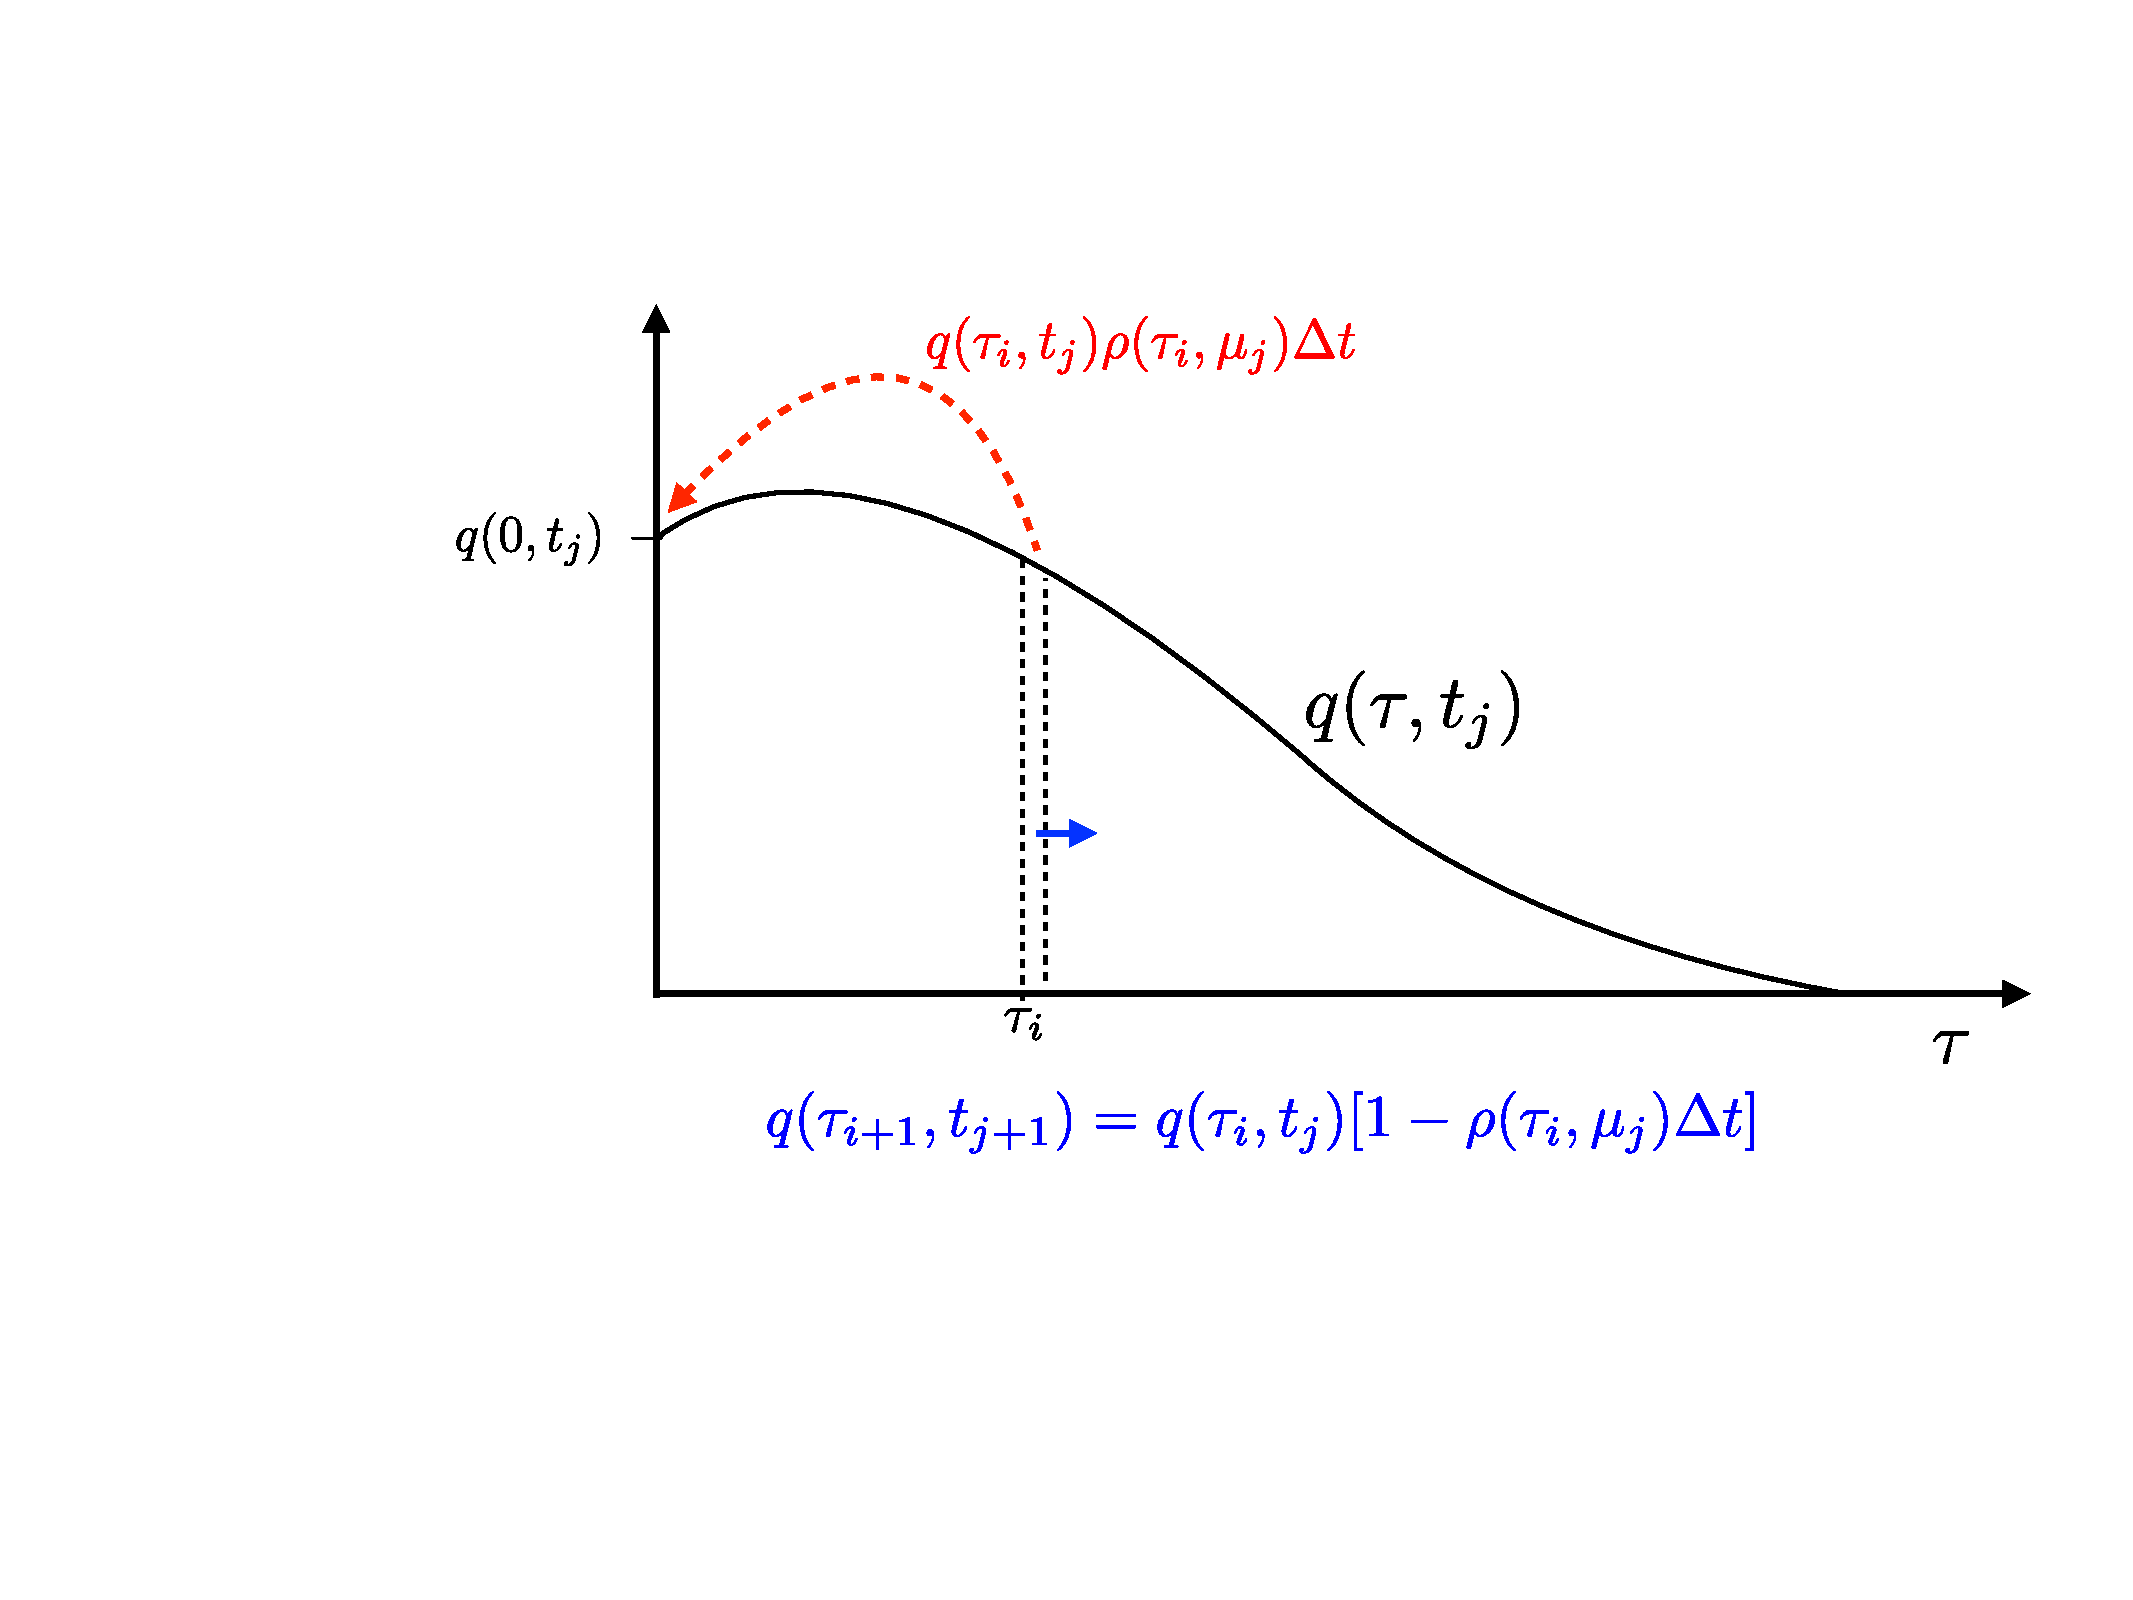
\includegraphics[width=70mm]{qtau}
	
\end{figure}


\pause
The refractory density $q(\tau,t)$ obeys the master equation:

\vspace{0.1cm}
\hspace{2.5cm}$
\partial_t q(\tau,t)+ \partial_\tau q(\tau,t)=-\rho(\tau,\mu)q(\tau,t)
$

\end{frame}


\setbeamerfont{frametitle}{size=\normalsize }
\begin{frame}
\frametitle{1.1 Refractory density equation}


 \begin{figure}
	\centering
	
	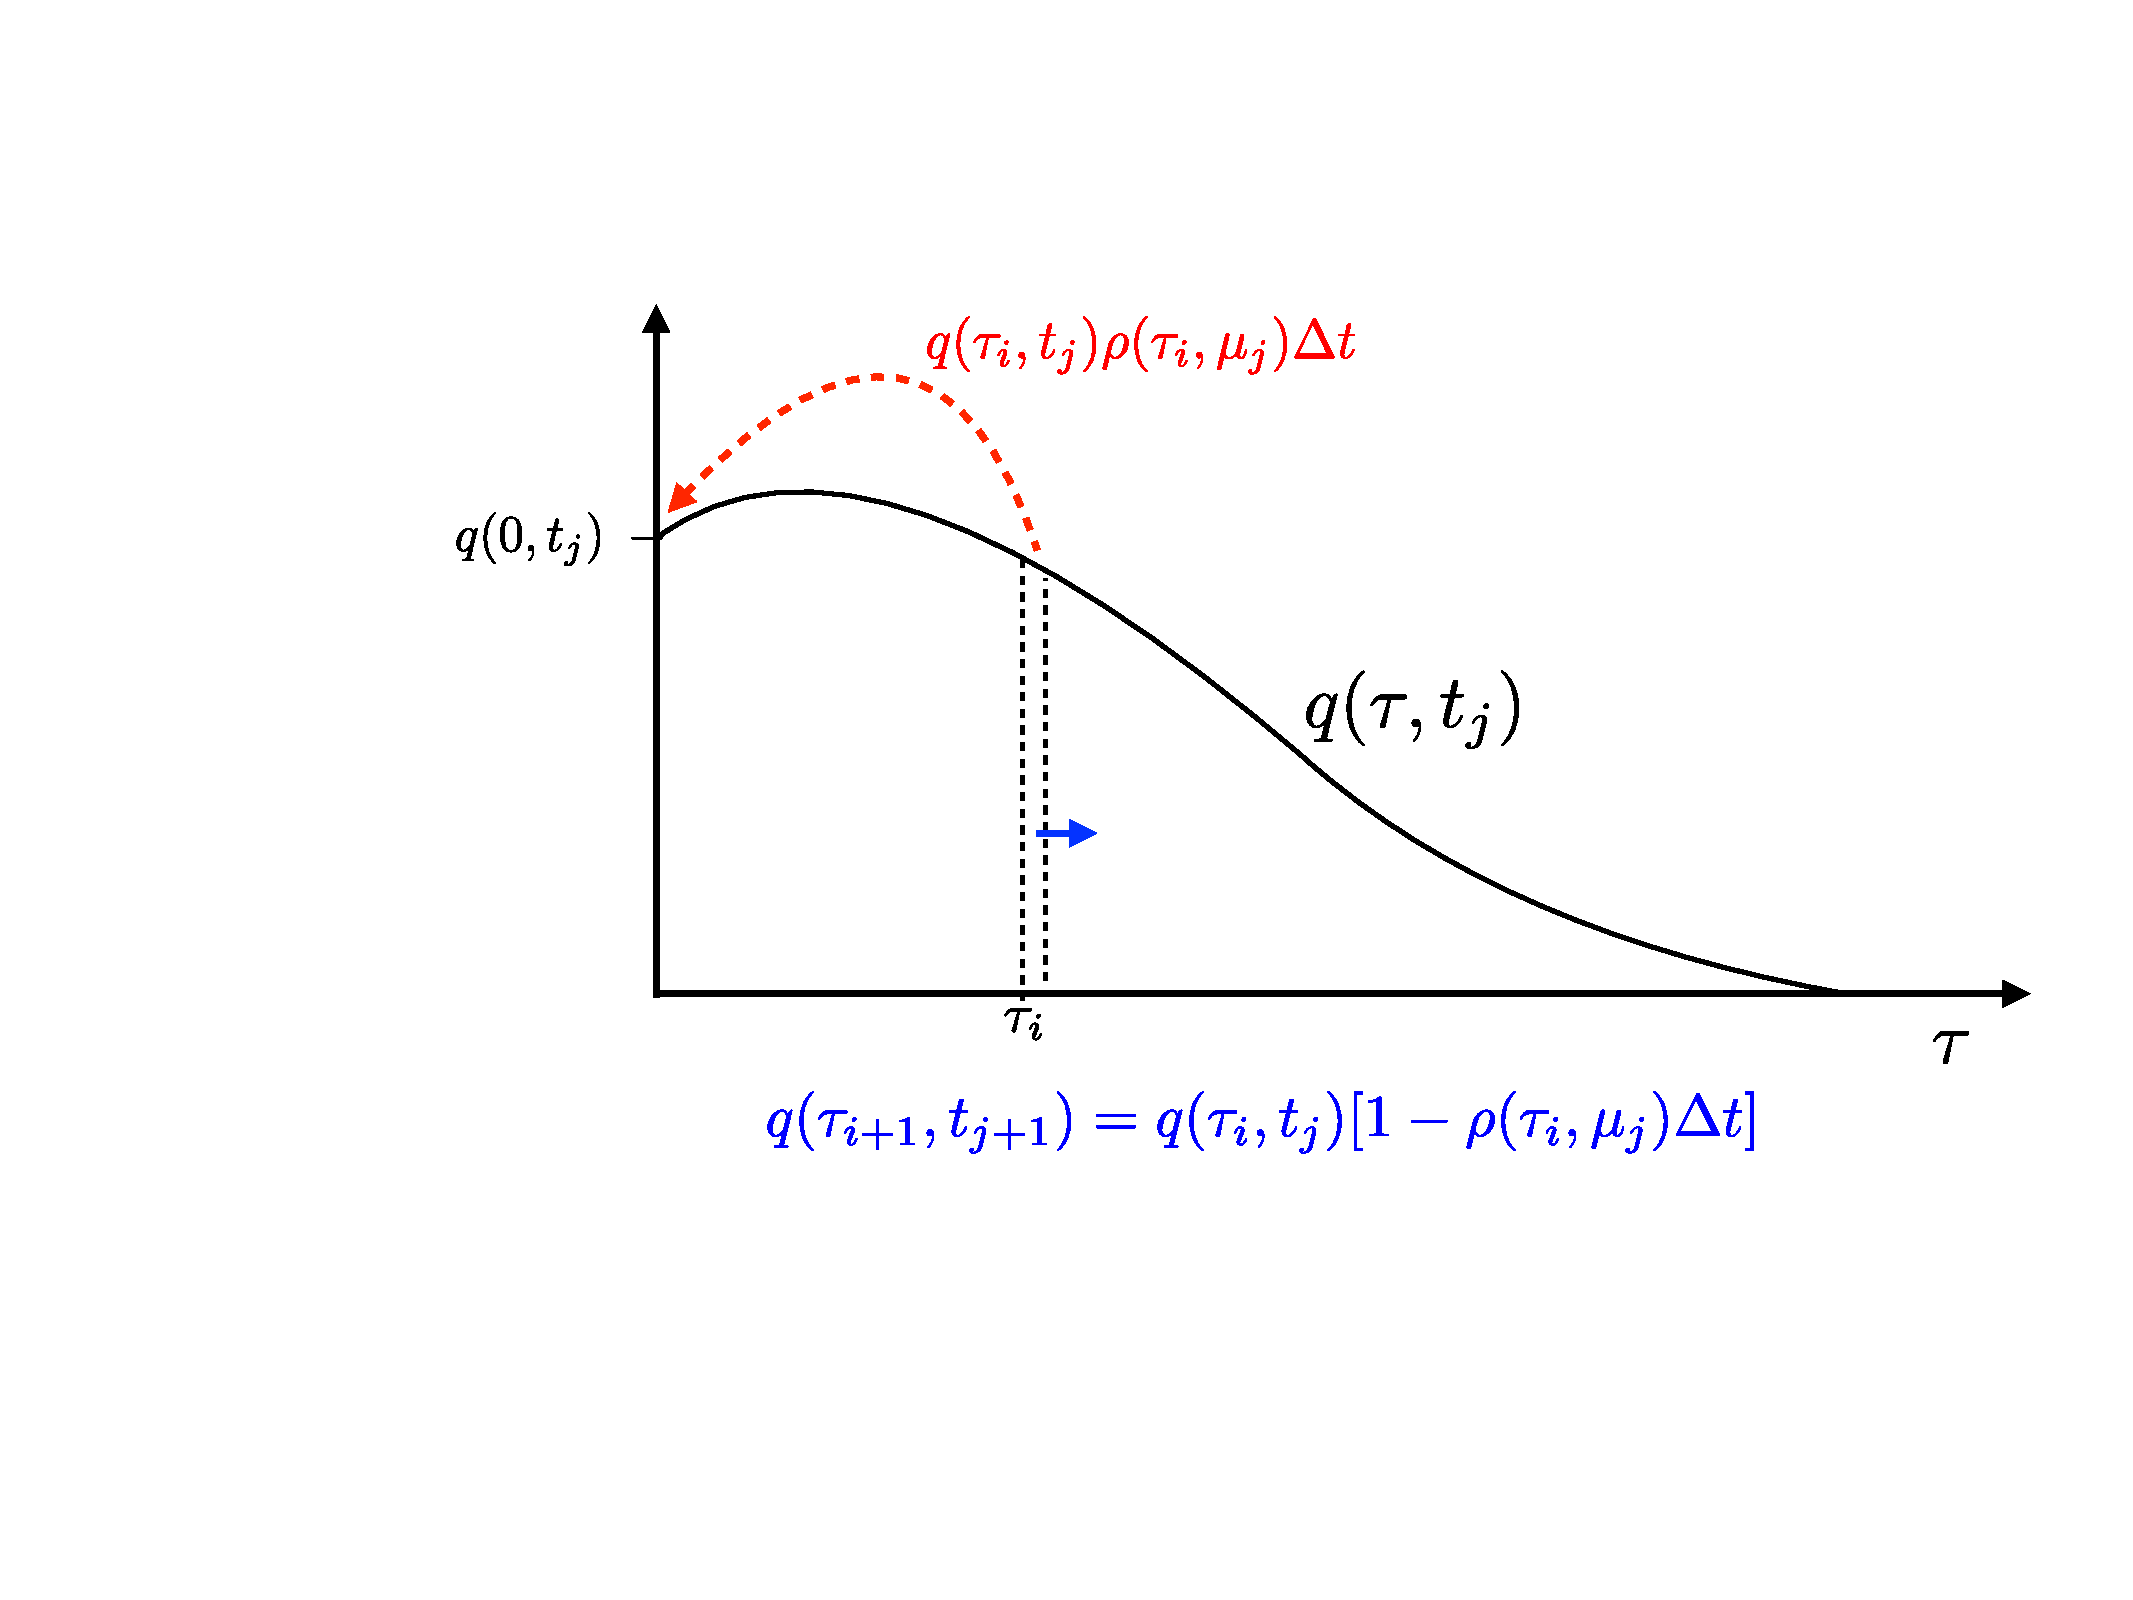
\includegraphics[width=70mm]{qtau}
	
\end{figure}


The refractory density $q(\tau,t)$ obeys the master equation:

\vspace{0.3cm}
\hspace{2.5cm}$
\partial_t q(\tau,t)+ \partial_\tau q(\tau,t)=-\rho(\tau,\mu)q(\tau,t)
$


\vspace{0.3cm}
With boundary conditions:
\begin{align}
\label{boundarycondition}
q(0,t)&=\int_{0}^{\infty}\rho(\tau,t)q(\tau,t)d\tau=A(t) \nonumber\\
q(\infty,t)&=0 \nonumber
\end{align}

\end{frame}


\subsection{1.2 Eigenfunction expansion of the refractory density}

\begin{frame}
\frametitle{1.2 Eigenfunction expansion of the refractory density}

We consider first the time homogeneous case: $\rho(\tau,\mu)=\rho(\tau)$

\vspace{0.2cm}
\hspace{2.9cm}
\begin{align*}
\partial_t q(\tau,t)&=-\partial_\tau q(\tau,t)-\rho(\tau)q(\tau,t) \\
&=\mathcal{L}\:q(\tau,t)
\end{align*}


\vspace{0.5cm}
\hspace{2.5cm}  with $\mathcal{L}=-\partial_{\tau}-\rho(\tau)$ 



\end{frame}


\begin{frame}
\frametitle{1.2 Eigenfunction expansion of the refractory density}



\hspace{1cm} $\partial_t q(\tau,t)=\mathcal{L}\:q(\tau,t)$ \hspace{1cm} with \hspace{1cm}  $\mathcal{L}=-\partial_{\tau}-\rho(\tau)$ 


\vspace{0.3cm}
We can expand the refractory density as:

\vspace{0.2cm}
\hspace{3.1cm}
$q(\tau,t)=\sum_n a_n(t)\phi_n(\tau) $

\pause
\vspace{0.3cm}
where $\phi_n(\tau)$ are the eigenfunctions of the operator $\mathcal{L}$

\vspace{0.2cm}
 \hspace{2.4cm} \hspace{1cm}$
\mathcal{L}\phi_n=\lambda_n\phi_n
$

\vspace{0.3cm}
With eigenvalues $\lambda_n$ and boundary conditions:
\begin{align}
\phi_n(0)&=\int_{0}^{\infty}\rho(\tau)\phi_n(\tau)d\tau \nonumber\\
\phi_n(\infty)&=0 \nonumber
\end{align}


\end{frame}


\begin{frame}
\frametitle{1.2 Eigenfunction expansion of the refractory density}

Solving $[-\partial_{\tau}-\rho(\tau)]\phi_n=\lambda_n\phi_n$ we have:

\vspace{0.2cm}

\hspace{1.8cm}$\phi_n(\tau)=\phi_n(0)\exp(-\lambda_n\tau-\int_0^\tau\rho(s)ds)$

\vspace{0.5cm}
\pause
Using the boundary condition we find:

\vspace{0.2cm}

\hspace{1.8cm}$\phi_n(0)=\int_0^{\infty}\rho(\tau)\phi_n(0)\exp(-\lambda_n\tau-\int_0^\tau\rho(s)ds)$

\vspace{0.5cm}
\pause
which can be written as:

\vspace{0.2cm}

\hspace{2.5cm}\fbox{$1=\int_0^{\infty}e^{-\lambda_n\tau}P(\tau)d\tau$}

\vspace{0.5cm}
with ISI density $P(\tau)=\rho(\tau) \exp(-\int_0^\tau\rho(s)ds)$

\vspace{0.5cm}
\pause
$\Rightarrow$ $\lambda_0=0$ fulfilled the condition, it corresponds to the stationary density


\end{frame}

\subsection{1.3 Definition and property of the adjoint operator $\mathcal{L}^+$}

\begin{frame}
\frametitle{1.3 Definition and property of the adjoint operator $\mathcal{L}^+$}

To recover the activity we will need the eigenfunctions $\psi_n$ of the adjoint operator $\mathcal{L}^+$:

\hspace{3.8cm}
$\mathcal{L}^+\psi_n=\lambda_n\psi_n$

\pause
\vspace{0.5cm}
Defining the inner product : $(\psi,\phi)=\int_{0}^{\infty}\psi(\tau)\phi(\tau)d\tau$

\vspace{0.5cm} and using the property: $(\psi,\mathcal{L}\phi)  = (\mathcal{L}^+\psi,\phi)$

\pause
\vspace{0.5cm} 
One can obtained the adjoint operator $\mathcal{L}^+$:


\vspace{0.2cm} 
\hspace{2cm}$
\mathcal{L}^+\psi(\tau)=[\partial_{\tau}-\rho(\tau)]\psi(\tau)+\psi(0)\rho(\tau)
$

\pause
\vspace{0.5cm} 
$\psi_n$, $\phi_n$ form a biorthonormal basis:
\vspace{0.3cm}
\hspace{3.8cm}
$
(\psi_i,\phi_j)=\delta_{ij}
$
\end{frame}


\subsection{1.4 Recover the Activity}
\begin{frame}
\frametitle{1.4 Recover the Activity}
The activity is given by:

\vspace{0.2cm}
\hspace{3cm} $A(t)=q(t,0)=\sum_n a_n(t)\phi_n(0) $

\pause
\vspace{0.5cm}
We derived $a_n(t)$ by projecting $q(\tau,t)$ on the eigenbasis:

\vspace{0.2cm}
\hspace{3cm}$ a_n(t)=(\psi_n,q)$

\pause
\vspace{0.5cm}
From which we obtained:

\begin{align*}
\frac{d a_n}{dt}&=(\psi_n,\partial_tq)  \\
&=(\psi_n,\mathcal{L}q)  \\
&=(\mathcal{L}^+\psi_n,q) \\
&=\lambda_na_n
\end{align*}

\vspace{0.2cm}
\hspace{3cm}$a_n(t) = a_n(0)\exp(\lambda_nt)$
%with \hspace{0.4cm} a_n(0) = & \int_{0}^{\infty}\psi_n(\tau)q(0,\tau)d\tau
%\end{align*}

\end{frame}

\begin{frame}
\frametitle{1.4 Recover the Activity}

The activity is given by:

\vspace{0.2cm}
\hspace{3cm} $A(t)=q(t,0)=\sum_n a_n(t)\phi_n(0) $

\vspace{0.5cm}
Keeping the two first modes, one can obtain a second order differential equation for the firing rate :

\vspace{0.2cm}
\hspace{3cm}$\ddot A(t)=[2Re(\frac{1}{\lambda_1})\dot A(t)-A(t)+A_{\infty}] |{\lambda_1}|^2$

\vspace{0.2cm}
\small{M. Mattia, \textit{Low-dimensional firing rate dynamic of spiking neuron networks} (2016)}

%\pause
%\vspace{0.3cm}
%In particular for initial condition $q(0,\tau)=\delta(\tau)$ we have:

%\vspace{0.2cm}
%\hspace{3.8cm}$A(t)=\sum_n \psi_n(0)\phi_n(0)\exp(\lambda_nt) $

\end{frame}

\setbeamerfont{frametitle}{size=\Large}

\subsection{2.5 Resume of the theoretical derivation}
\begin{frame}
\frametitle{2.5 Resume of the theoretical derivation}

We can expand the refractory density as:

\vspace{0.2cm}
\hspace{3.1cm}
$q(\tau,t)=\sum_n a_n(t)\phi_n(\tau) $

\pause
\vspace{0.3cm}
from this expansion we found a condition for the eigenvalues $\lambda_n$:
\hspace{2.5cm}\fbox{$1=\int_0^{\infty}e^{-\lambda_n\tau}P(\tau)d\tau$}

\pause
\vspace{0.3cm}
Knowing the eigenvalues and the hazard function we can analytically define the eigenfunctions $\phi_n$ and $\psi_n$.

\pause
\vspace{0.3cm}
Thanks to those eigenfunctions we can recover the activity: %n particular starting with initial condition $q(0,\tau)=\delta(\tau)$ :

\vspace{0.2cm}
\hspace{3.cm}$A(t)=\sum_n a_n(t)\phi_n(0) $%$A(t)=\sum_n \psi_n(0)\phi_n(0)\exp(\lambda_nt) $

\end{frame}


\begin{frame}
\frametitle{Overview}% Table of contents slide, comment this block out to remove it
\tableofcontents % Throughout your presentation, if you choose to use \section{} and \subsection{} commands, these will automatically be printed on this slide as an overview of your presentation
\end{frame}

\section{2 Spectral expansion for different processes}

\subsection{2.1 Gamma process}
\begin{frame}
\frametitle{2 Spectral expansion for different processes}
\framesubtitle{2.1 Gamma process}

The ISI distribution is given by: 	

\vspace{0.2cm}
\hspace{2.5cm}$P(\tau)=\frac{\beta^\gamma}{(\gamma-1)!}\tau^{\gamma-1}e^{-\beta\tau}$ for integer $\gamma$ and $\beta>0$. 

\pause
\vspace{0.3cm}
The Laplace transform can be derived analytically:

\vspace{0.2cm}
\hspace{2.5cm}$\bar{P}(\lambda)=(\frac{\beta}{\beta+\lambda})^\gamma$

\pause
\vspace{0.3cm}
Solving $\bar{P}(\lambda_n)=1$ we find:

\vspace{0.2cm}
\hspace{2.8cm} $\lambda_n=\beta(\exp(\frac{2\pi i}{\gamma}n)-1)$, $n=0,..., \gamma-1$

\end{frame}

\begin{frame}

\frametitle{2.1 Gamma process}
\small{Initial condition $q(\tau,0)=\delta(\tau)$ $\rightarrow$ $A(t)=\sum_{n=0}^{\gamma-1}\psi_n(0)\phi_n(0)exp(\lambda_nt)$}
\begin{figure}
		\centering
	
	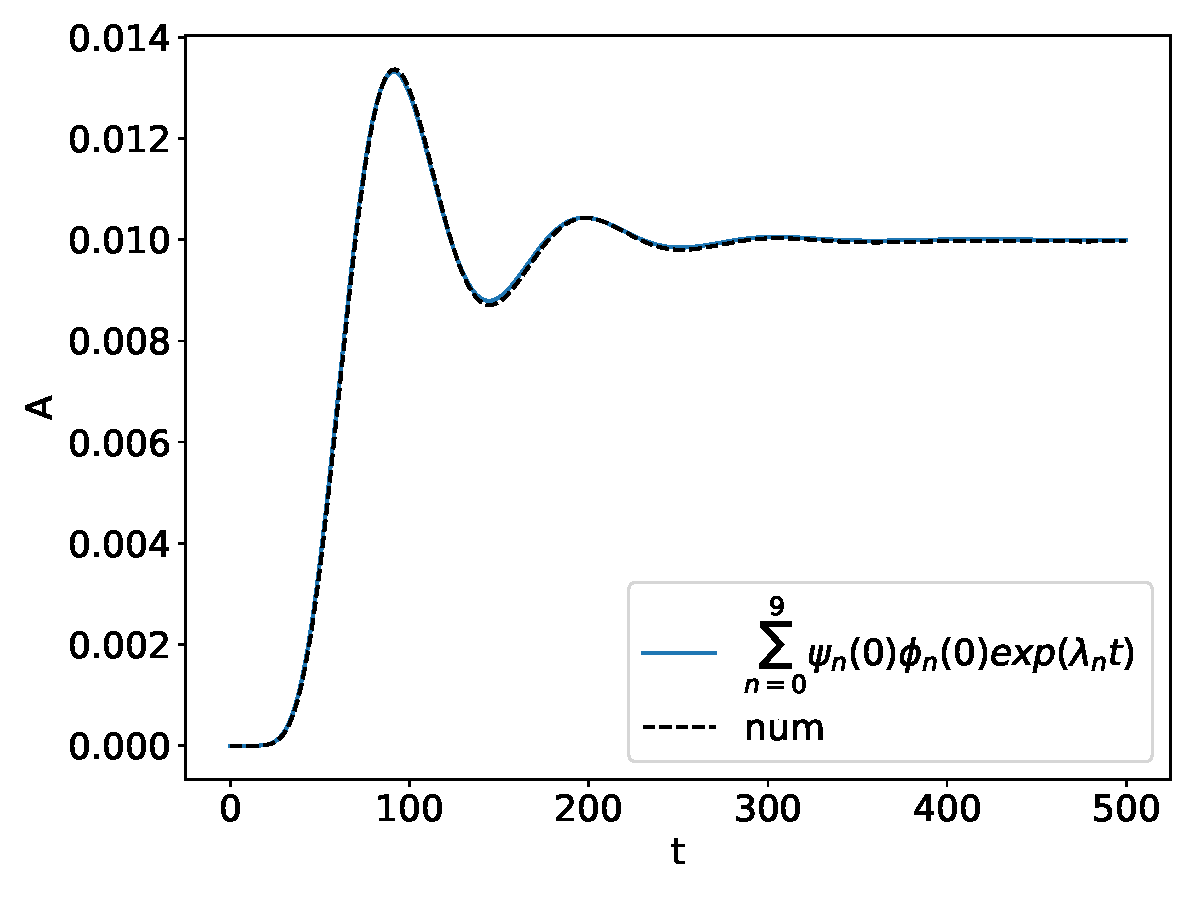
\includegraphics[width=70mm]{sum10gamma.pdf}


$\beta=0.1$, $\gamma=10$
\end{figure}


\end{frame}



\subsection{2.2 Inverse Gaussian process}

\begin{frame}
\frametitle{2.2 Inverse Gaussian process}
The perfect integrate fire model driven by a Gaussian white noise:

\vspace{0.3cm}
$\dot V=\mu +\sqrt{2D}\xi(t)$ \hspace{1cm} $<\xi(t)\xi(s)>=\delta(t-s)$

\vspace{0.2cm}
if $V=V_{th}:\:V\rightarrow V_r$

\begin{figure}
	\centering
	
	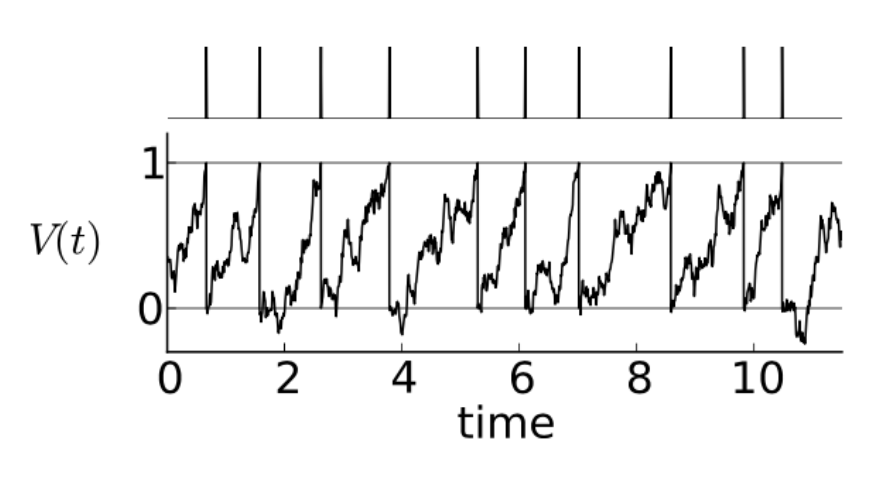
\includegraphics[width=70mm]{tilo}
	
	
	\small{$\mu=1$, $D=0.125$ and $V_{th}=1$}\\
	\tiny{
		\textit{figure: T. Schwalger, The interspike-interval statistics of non-renewal neuron models (2013) }}
	
\end{figure}

\end{frame}

\begin{frame}
\frametitle{2.2 Inverse Gaussian process}
The ISI distribution is given by: 	

\vspace{0.2cm}
\hspace{2.5cm}$P(\tau)=\frac{V_{th}}{\sqrt{4\pi D\tau^3}}\exp(-\frac{(\mu\tau-V_{th})^2}{4D\tau})$


\pause
\vspace{0.3cm}
The Laplace transform can be derived analytically:

\vspace{0.2cm}
\hspace{2.5cm}$\bar{P}(\lambda)=\exp(\frac{\mu V_{th}}{2D}[1-\sqrt{1+\frac{4D\lambda}{\mu^2}}])$

\pause
\vspace{0.3cm}
Solving $\bar{P}(\lambda_n)=1$ we find:

\vspace{0.2cm}
\hspace{2.8cm} $\lambda_n=- \frac{2\pi\mu}{V_{th}}n( \frac{2\pi D}{\mu V_{th}}n + i)$



\end{frame}

\begin{frame}
\frametitle{2.2 Inverse Gaussian process}

Recover the activity solving the  second order differential equation:

\hspace{3cm} $\ddot A(t)=[2Re(\frac{1}{\lambda_1})\dot A(t)-A(t)+A_{\infty}] |{\lambda_1}|^2$

\begin{figure}
\centering

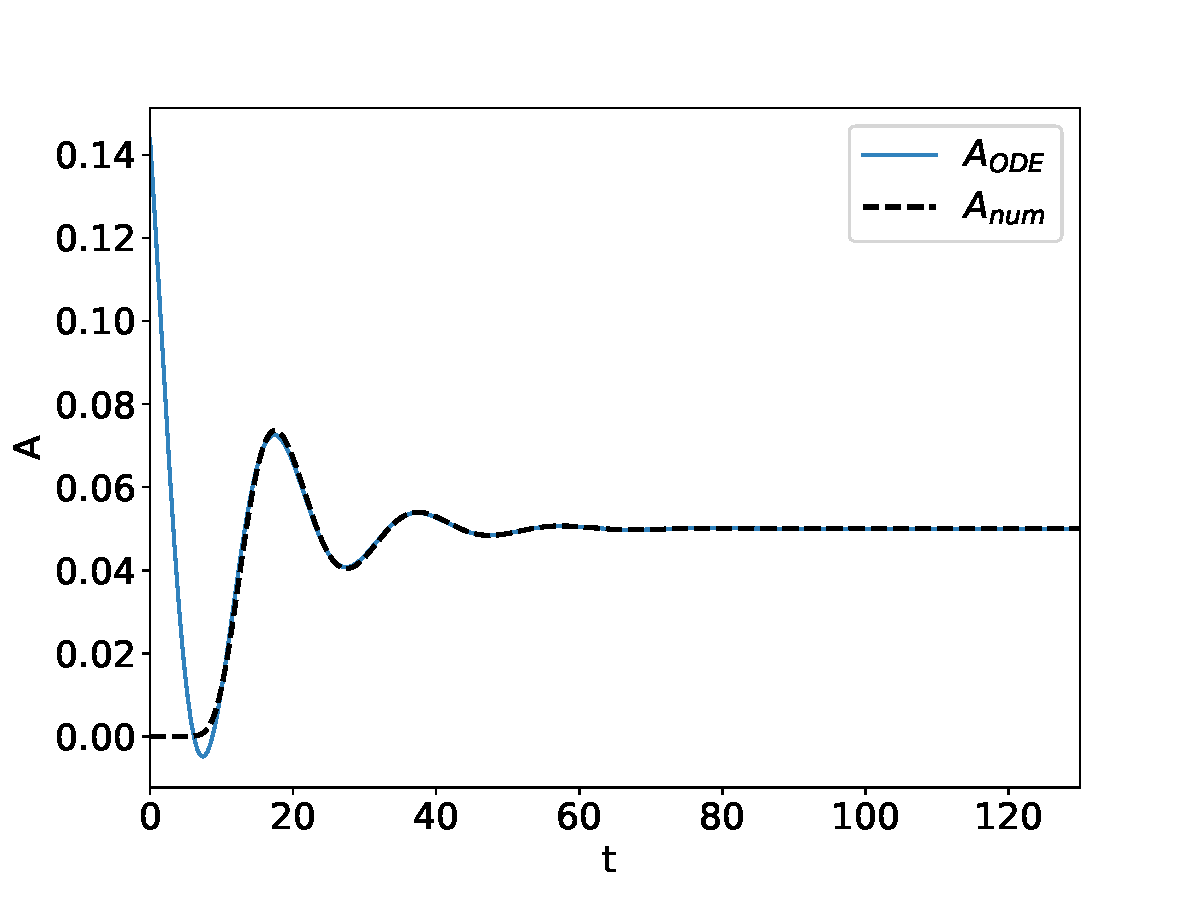
\includegraphics[width=70mm]{AODE.pdf}

\vspace{0.5cm}
\small{$\mu=0.05$ ,$D=0.002$, $V_{th}=1$}

\end{figure}



\end{frame}




\section{4. Summary and Future Work}
\begin{frame}
\begin{itemize}
	\frametitle{4. Summary and Future Work}
	\item 	We made an expansion of the refractory density for time homogeneous hazard rates $\rho(\tau,\mu)=\rho(\tau)$ 
	\pause
	\item We obtained a low dimensional dynamics for the firing rate in the case of uncoupled neuron
\end{itemize}
\pause
Future work:
\begin{itemize}
	
	\item Derive a low-dimensional ordinary differential equation for the firing rate in the case of a coupled network.
	
	\vspace{0.1cm}
	\hspace{2cm} $\frac{d a_n}{dt}= \lambda_na_n+\frac{d\mu}{dt}(\frac{\partial \psi_n}{\partial \mu},q)$
	\pause
	\item Find a efficient method to approximate the first eigenvalue for any hazard rate $\rho(\tau,\mu)$
	
		\vspace{0.1cm}
		\hspace{2.4cm} $1=\int_0^{\infty}e^{-\lambda_n\tau}P(\tau)d\tau$


\end{itemize}




\end{frame}

\begin{frame}

\hspace{2cm} \Large{Thanks for your attention}

\end{frame}


%\subsection{3.2 Gamma process}




\begin{frame}
 one can show that for different eigenvalues, the eigenfunctions $\psi_i$ and $\phi_j$ are orthogonal:
\begin{align}
\lambda_j(\psi_i,\phi_j) 
&=(\psi_i,\mathcal{L}\phi_j) \nonumber \\
&=(\mathcal{L}^+\psi_i,\phi_j)  \nonumber \\
&=\lambda_i(\psi_i,\phi_j) \nonumber
\end{align}

\end{frame}


\begin{frame}
\frametitle{2.2 Definition and property of the adjoint operator $\mathcal{L}^+$}

\begin{align}
(\psi,\mathcal{L}\phi)&= \int_{0}^{\infty}\psi(\tau)\mathcal{L}\phi(\tau)d\tau  \nonumber \\
&= \int_{0}^{\infty}\psi(\tau)[-\partial_{\tau}-\rho(\tau)]\phi(\tau)d\tau  \nonumber \\
&=-[\psi(\tau)\phi(\tau)]^{\infty}_{0}+\int_{0}^{\infty}\partial_{\tau}\psi(\tau)\phi(\tau)d\tau -\int_{0}^{\infty}\rho(\tau)\psi(\tau)\phi(\tau)d\tau \nonumber \\
&= \psi(0)\phi(0)+ \int_{0}^{\infty}[\partial_{\tau}-\rho(\tau)]\psi(\tau)\phi(\tau)d\tau  \nonumber \\
&=\int_{0}^{\infty} \psi(0)\rho(\tau)\phi(\tau)d\tau+ \int_{0}^{\infty}[\partial_{\tau}-\rho(\tau)]\psi(\tau)\phi(\tau)d\tau  \nonumber \\
&= \int_{0}^{\infty}\{[\partial_{\tau}-\rho(\tau)]\psi(\tau)+ \psi(0)\rho(\tau)\}\phi(\tau)d\tau  \nonumber \\
& = (\mathcal{L}^+\psi,\phi) \nonumber
\end{align}

with 
$
\mathcal{L}^+\psi(\tau)=[\partial_{\tau}-\rho(\tau)]\psi(\tau)+\psi(0)\rho(\tau)
$
\end{frame}

\begin{frame}
\frametitle{2.2 Definition and property of the adjoint operator $\mathcal{L}^+$}
\begin{align*}
\mathcal{L}^+\psi_n(\tau)&=[\partial_{\tau}-\rho(\tau)]\psi_n(\tau)+\psi_n(0)\rho(\tau)\\
&=\lambda_n\psi_n(\tau)
\end{align*}

The solution of this equation is:

\vspace{0.2cm}

$
\psi_n(\tau)=\psi_n(0)\exp(\lambda_n\tau)S^{-1}(\tau)\big[1-\int^\tau_0 P(x) \exp\big(-\lambda_nx)dx\big] \nonumber
$


\end{frame}

\begin{frame}
\begin{align*}
1=&\int_0^{\infty}\phi_n(0)\psi_n(0)\big[1-\int^\tau_0 P(x) \exp\big(-\lambda_nx)dx\big]d\tau \\
\phi_n(0)\psi_n(0) =&\frac{1}{\int_0^{\infty}\big[1-\int^\tau_0 P(x) \exp\big(-\lambda_nx)dx\big]d\tau}
\end{align*}
\end{frame}

\begin{frame}
\frametitle{ Second order differential equation for the firing rate for uncoupled neurons}

\vspace{1cm}
M. Mattia, \textit{Low-dimensional firing rate dynamic of spiking neuron networks} (2016)

\vspace{1cm}

\hspace{1cm}$\ddot A(t)=[2Re(\frac{1}{\lambda_1})\dot A(t)-A(t)+A_{\infty}] |{\lambda_1}|^2$

\end{frame}


\end{document}